\subsection{Problem setup}

The policy receives RGB observations from one or more cameras, proprioception, and optionally camera-pose labels for a subset of training examples. It predicts an action chunk for imitation learning. The central design choice is whether camera geometry is supplied as fixed calibration, predicted by a separate model, or optimized jointly with the action policy.

\subsection{Semi-supervised camera-pose prediction}

The camera-pose predictor maps observations to camera poses or equivalent pose/ray parameters. Only a subset of training examples require ground-truth camera-pose labels. The supervised pose loss anchors the prediction, while the downstream action objective continues to shape the representation used by the policy. This setup treats pose prediction as part of the control system rather than as a fixed preprocessing step.

\subsection{E2E camera-pose action policy}

The action-only variant predicts camera geometry, converts it into pose or ray tokens, and conditions an observation encoder on those tokens. The action expert then predicts action chunks from the encoded observation representation. Its training objective is
\begin{equation}
  \mathcal{L}_{\mathrm{action}} + \lambda_{\mathrm{pose}}\mathcal{L}_{\mathrm{pose}}.
\end{equation}

\subsection{E2E camera-pose NVS policy}

The NVS variant uses a register-style observation encoder. Its latent registers are consumed by both an action expert and a novel-view synthesis decoder. During training, the NVS decoder receives a target camera pose or ray query and reconstructs a held-out target view. The resulting training objective is
\begin{equation}
  \mathcal{L}_{\mathrm{action}} +
  \lambda_{\mathrm{pose}}\mathcal{L}_{\mathrm{pose}} +
  \lambda_{\mathrm{nvs}}\mathcal{L}_{\mathrm{nvs}}.
\end{equation}
The rendering head is used only during training. At inference, the model uses predicted camera geometry and the action expert.

\begin{figure}[t]
  \centering
  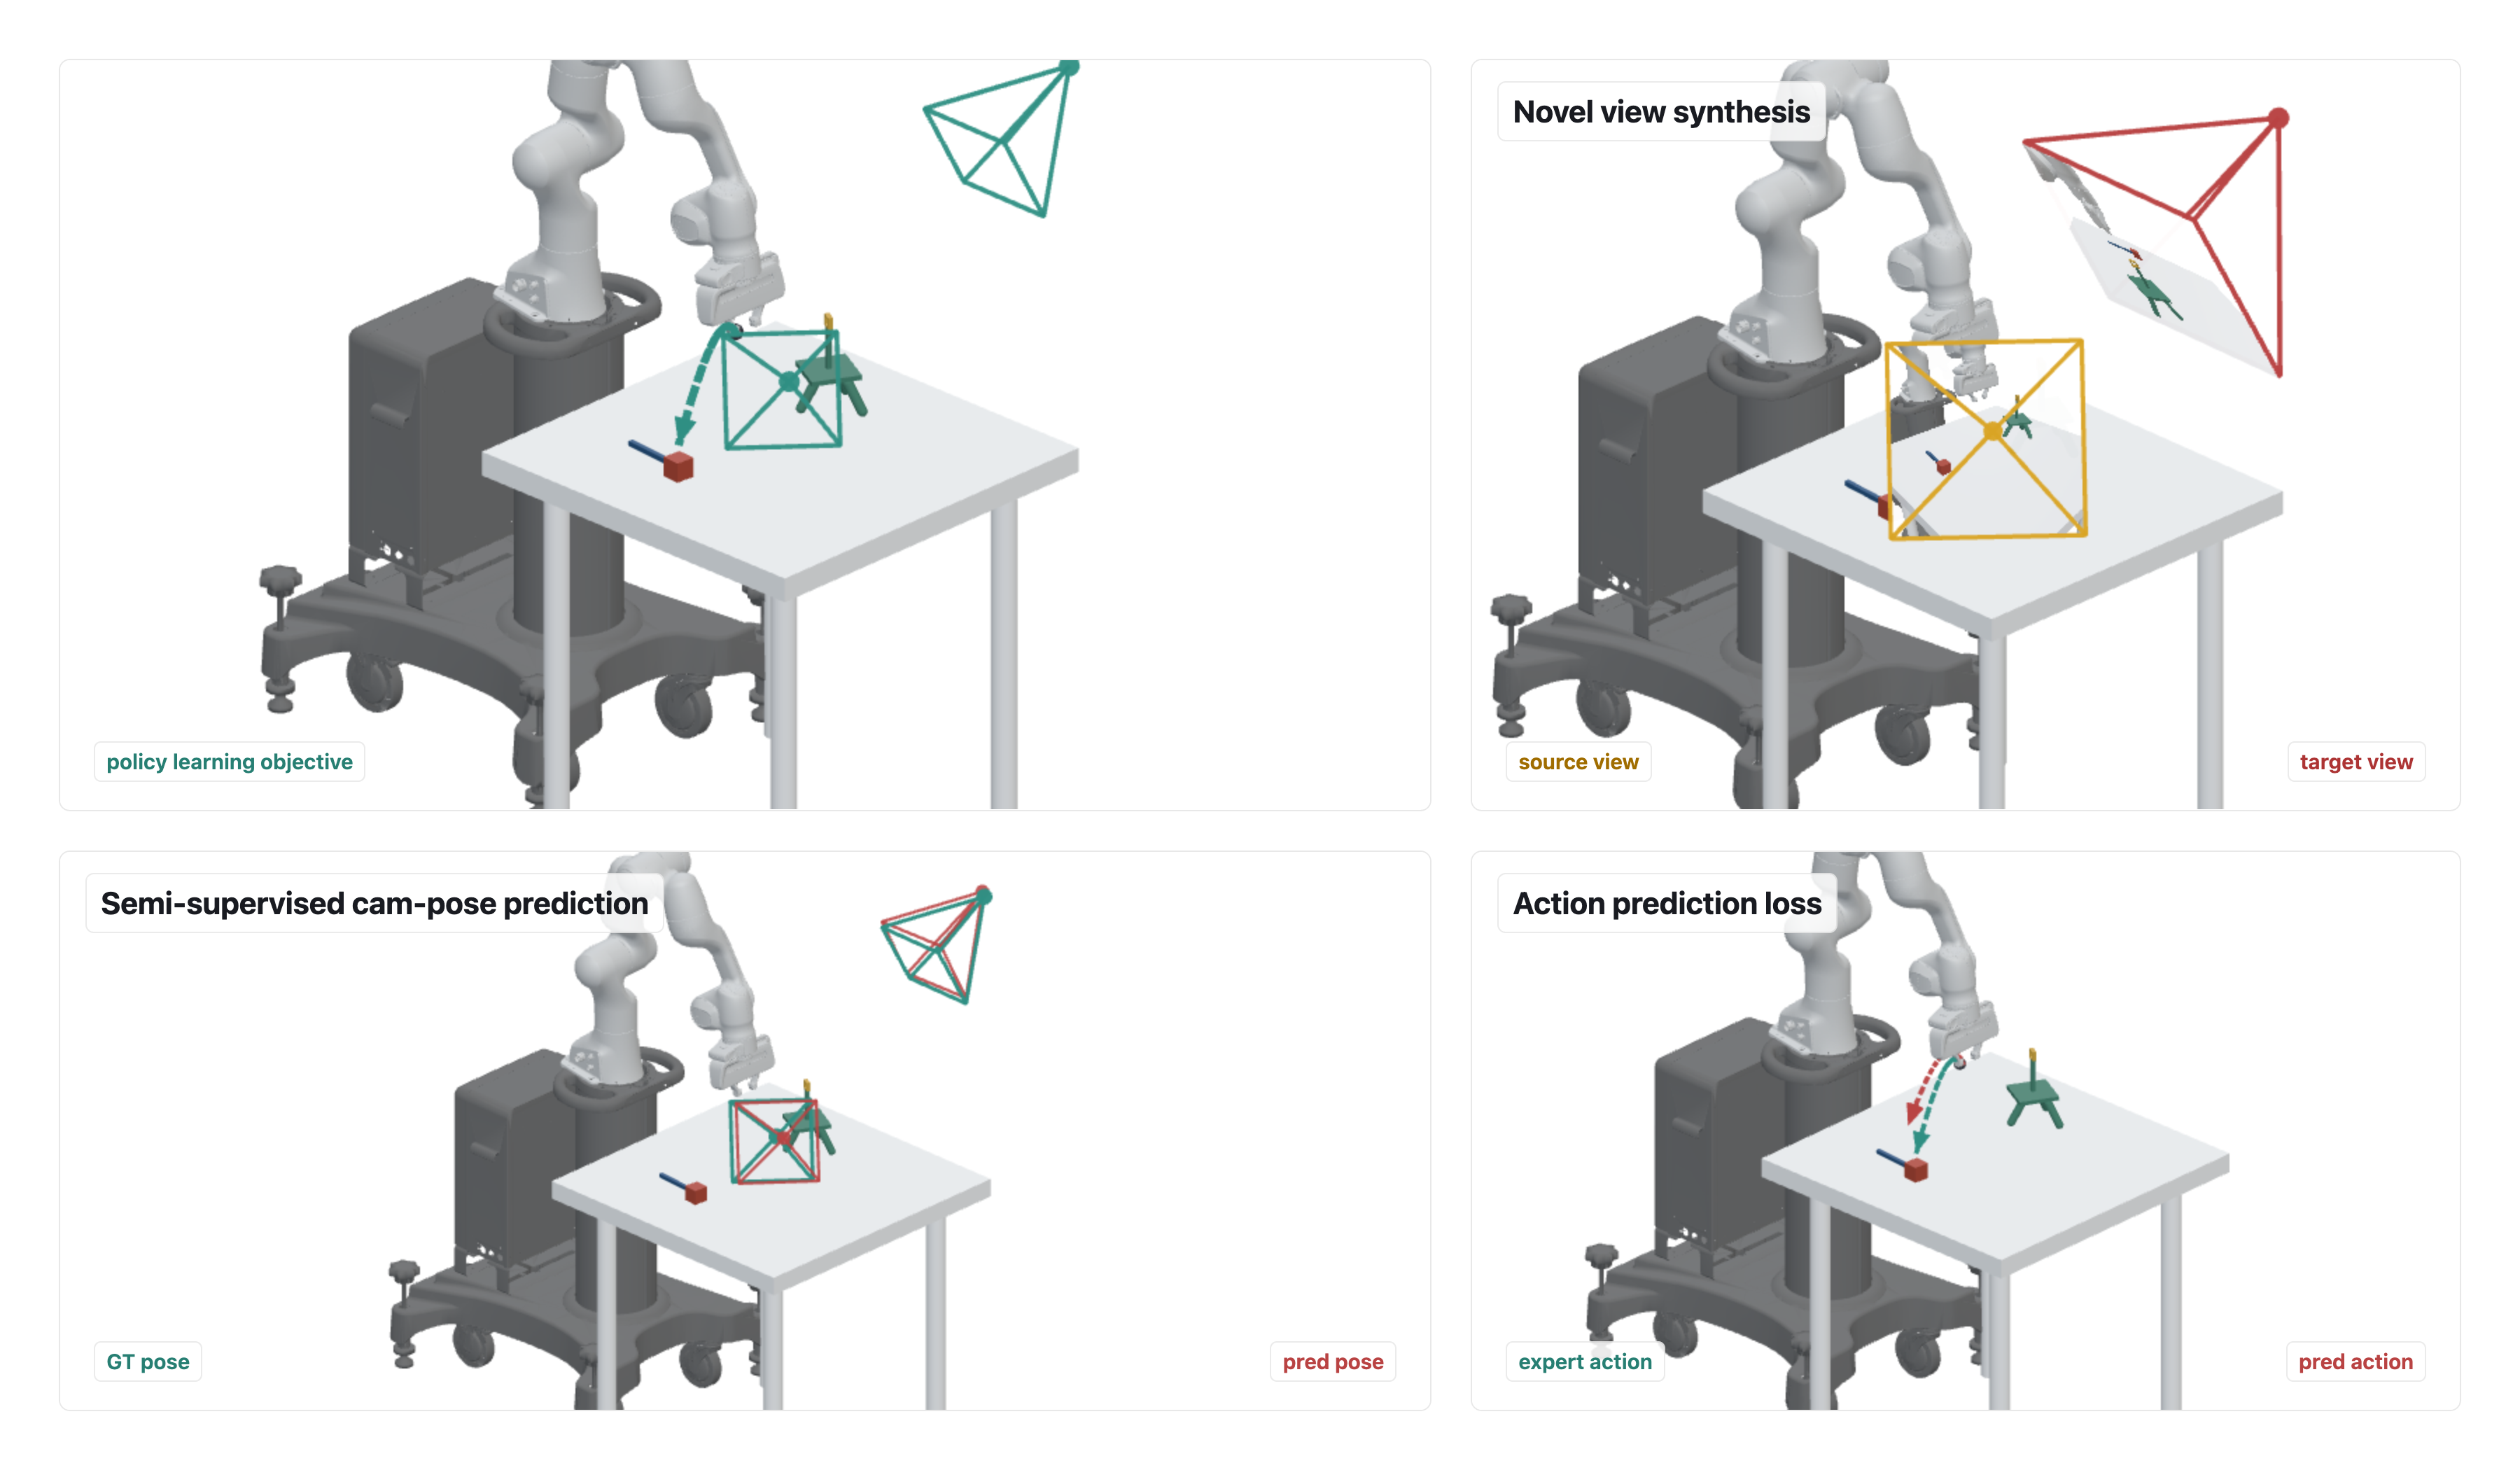
\includegraphics[width=\linewidth]{figures/teaser.png}
  \caption{Draft teaser figure for the MimicGen setting, showing policy learning, pose prediction, novel-view synthesis, and action loss in the rendered evaluation scene.}
  \label{fig:teaser}
\end{figure}
